\documentclass{ximera}

\author{Bart Snapp}

\title{Sphere and circles}

\begin{document}
\begin{abstract}
  One group member will plot a sphere with two circles on it.
\end{abstract}
\maketitle

One group member will produce a plot like this one:
\begin{image}
  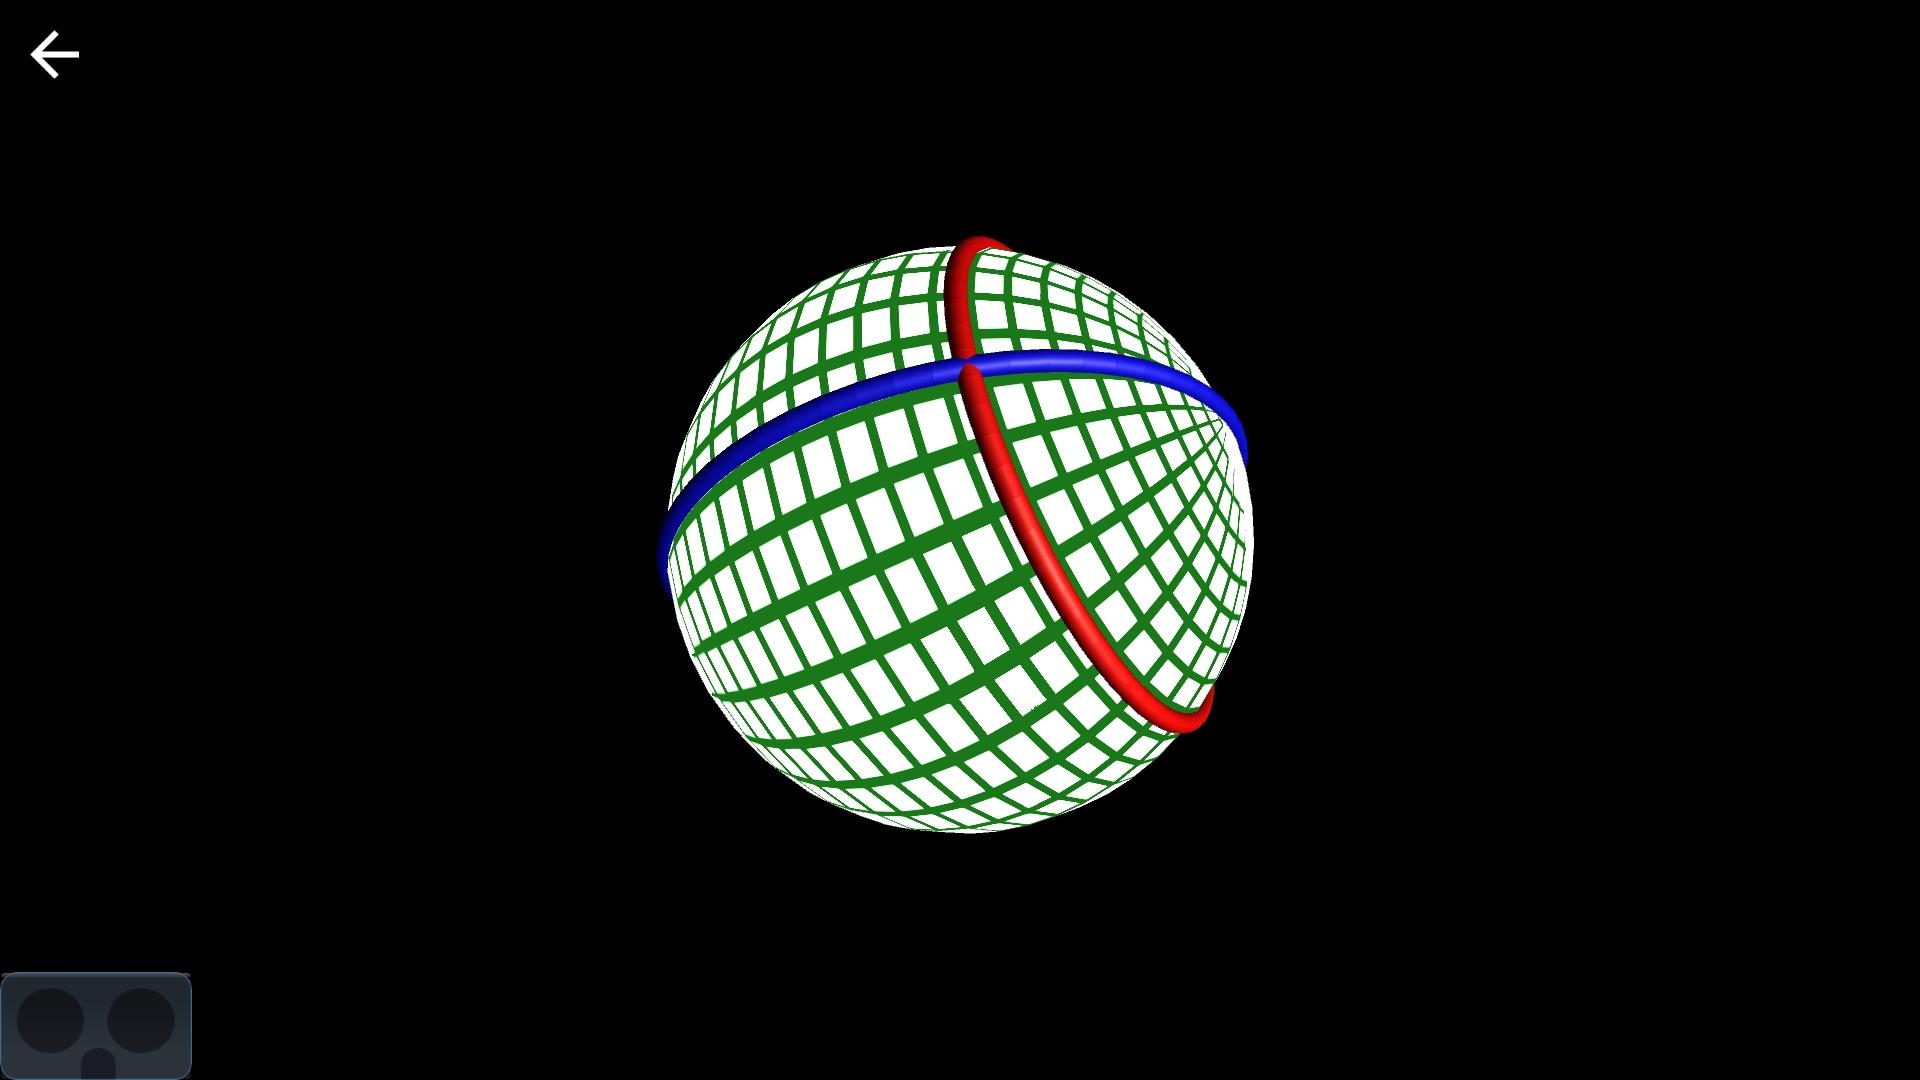
\includegraphics{sphereAndCircles.png}
\end{image}

This is a sphere of radius $3$ with two circles on it:
\begin{itemize}
\item A great circle. Read more about great circles \link[here]{https://en.wikipedia.org/wiki/Great_circle}.
\item A regular (non-great) circle. Read more about circles on a sphere \link[here]{https://en.wikipedia.org/wiki/Circle_of_a_sphere}.
\end{itemize}

As a gesture of friendship, I will tell you that the parametric
formula for a sphere of radius $R$ is:
\begin{align*}
  x(s,t) &= R\cdot \cos(t)\sin(s)\\
  y(s,t) &= R\cdot \sin(t)\sin(s)\\
  z(s,t) &= R\cdot \cos(s),
\end{align*}
where $0\le t< 2\pi$ and $0\le s \le \pi$.

You may color you circles any color you like---though you must make
them \textbf{different} colors.
\end{document}
